\documentclass[tikz,border=6pt]{standalone}
\usepackage[T1]{fontenc}
\usepackage{lmodern}
\usepackage{amsmath,amssymb}
\usetikzlibrary{arrows.meta,angles,quotes,calc,positioning}
\definecolor{axis}{HTML}{40515F}
\definecolor{grid}{HTML}{DDE4E8}
\definecolor{blue}{HTML}{3568D4}
\definecolor{coral}{HTML}{EF626C}
\definecolor{teal}{HTML}{2A9D8F}
\definecolor{gold}{HTML}{D89432}
\definecolor{purple}{HTML}{7357C8}
\tikzset{
  axisline/.style={axis, line width=.85pt, -{Stealth[length=3mm]}},
  guide/.style={axis!45, line width=.75pt, dashed},
  vector/.style={line width=1.5pt, -{Stealth[length=3mm]}},
  dot/.style={circle, fill=white, draw, line width=1.15pt, inner sep=2.15pt},
  label/.style={font=\large},
  smalllabel/.style={font=\normalsize}
}
\begin{document}

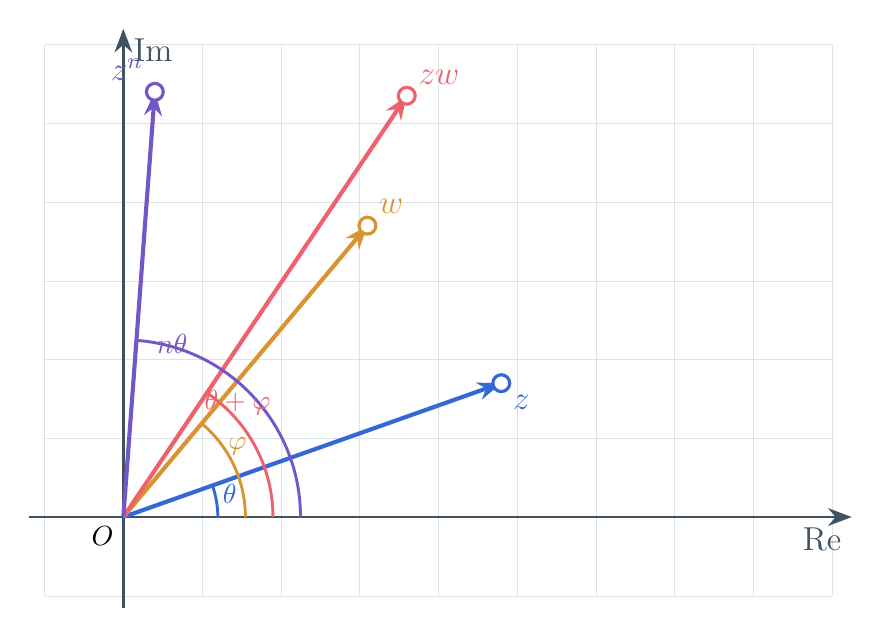
\begin{tikzpicture}[x=1cm,y=1cm]
  \draw[step=1cm,grid,very thin] (-1,-1) grid (9,6);
  \draw[axisline] (-1.2,0)--(9.25,0) node[below left,font=\large] {$\operatorname{Re}$};
  \draw[axisline] (0,-1.15)--(0,6.2) node[below right,font=\large] {$\operatorname{Im}$};
  \coordinate (O) at (0,0);
  \coordinate (Z) at (4.8,1.7);
  \coordinate (W) at (3.1,3.7);
  \coordinate (ZW) at (3.6,5.35);
  \coordinate (ZN) at (0.4,5.4);
  \draw[vector,blue] (O)--(Z);
  \draw[vector,gold] (O)--(W);
  \draw[vector,coral] (O)--(ZW);
  \draw[vector,purple] (O)--(ZN);
  \draw[blue,line width=1.05pt] (1.2,0) arc[start angle=0,end angle=19.5,radius=1.2];
  \draw[gold,line width=1.05pt] (1.55,0) arc[start angle=0,end angle=50,radius=1.55];
  \draw[coral,line width=1.05pt] (1.9,0) arc[start angle=0,end angle=56,radius=1.9];
  \draw[purple,line width=1.05pt] (2.25,0) arc[start angle=0,end angle=85.8,radius=2.25];
  \node[dot,draw=blue] at (Z) {};
  \node[dot,draw=gold] at (W) {};
  \node[dot,draw=coral] at (ZW) {};
  \node[dot,draw=purple] at (ZN) {};
  \node[label,blue,below right=1pt of Z] {$z$};
  \node[label,gold,above right=1pt of W] {$w$};
  \node[label,coral,above right=1pt of ZW] {$zw$};
  \node[label,purple,above left=1pt of ZN] {$z^n$};
  \node[smalllabel,blue] at (1.35,.3) {$\theta$};
  \node[smalllabel,gold] at (1.45,.9) {$\varphi$};
  \node[smalllabel,coral] at (1.45,1.45) {$\theta+\varphi$};
  \node[smalllabel,purple] at (.62,2.2) {$n\theta$};
  \node[smalllabel,below left] at (O) {$O$};
\end{tikzpicture}
\end{document}
